\subsection{Choques Rotacionais}

Conforme descrito na Metodologia, o primeiro dado a ser calculado é o Momento de Inércia da peça 2 conforme sua configuração geométrica e sua massa. Para realizar esse cálculo, utilizaremos a seguinte expressão para corpos cilíndricos ocos:

\[I_{CM} = \frac {1}{2}M(R_1^2+R_2^2)\]

sendo que:\\

\begin{table}[H]
    \centering
    \begin{tabular}{ |M{4.3cm}||M{1.7cm}||M{2cm}||M{2cm}|  }
        \hline
        \textbf{O que foi medido} & \textbf{Valor} & \textbf{Incerteza} & \textbf{Unidade}\\
        \hline
        Massa (M)               & 2,2429    & $\pm$ 0,0001  & kg\\
        Raio peça menor ($R_1$) & 0,0325    & $\pm$ 0,0001  & m\\
        Raio peça maior ($R_2$) & 0,0600    & $\pm$ 0,0001  & m\\
        \hline
    \end{tabular}
    \caption{Dados experimentais do Choque Rotacional}
\end{table}

Para o cálculo direto do Momento de Inércia da peça temos então:

\[I_{CM2} = \frac{1}{2} \cdot 2,2429 \cdot (0,0325^2+0,0600^2) = 1,12145 \cdot (0,00105625 + 0,0036)\]
\[I_{CM2} = 1,12145 \cdot (0,00465625)\]
\[I_{CM2} = 0,0052217516 (kg.m^2)\]

Agora, resta calcular a incerteza experimental envolvida na aferição das medidas. Para isso, devemos utilizar as regras já conhecidas para propagação de incerteza, respeitando a hierarquia dos cálculos. Primeiramente, calculamos a incerteza envolvida em uma potência:

\[\Delta R_1^2 = 2 \cdot R_1 \cdot \Delta R = 2 \cdot 0,0325 \cdot 0,0001 = 0,0000065\]
\[\Delta R_2^2 = 2 \cdot R_2 \cdot \Delta R = 2 \cdot 0,0600 \cdot 0,0001 = 0,0000120\]\

Feito essa etapa, a próxima envolvida é a soma de R12 e R22, então basta somar as incertezas de ambas calculadas:

\[\Delta (R_1^2 + R_2^2) = \Delta R_1^2 + \Delta R_2^2 = 0,0000065 + 0,0000120 = 0,0000185\]\

Por fim, basta calcular a incerteza envolvida no produto da massa M pela soma $R_1^2$ + $R_2^2$, não esquecendo da constante $1/2$ envolvida. Chamando de $\Delta z$ a incerteza propagada, temos:

\[\Delta z = \frac {1}{2}\cdot[M\cdot \Delta(R_1^2 + R_2^2) + (R_1^2 + R_2^2)\cdot M\]
\[\Delta z = \frac {1}{2}\cdot[2,2429\cdot 0,0000185 + 0,00465625\cdot 0,0001]\]
\[\Delta z = \frac {1}{2}\cdot[0,0000414937 + 0,0000004656] =\frac {1}{2}\cdot[0,0000419593] \]
\[\Delta z = 0,0000209797 = 0,00002 (kg.m^2)\]\

Portanto, respeitando os algarismos significativos, temos que o Momento de Inércia da Peça 2 com sua respectiva incerteza experimental é:

\[\therefore \mathbf{I_2 = (0,00522 \pm 0,00002) kg.m^2}\]\

Antes de analisar os dados dos choques rotacionais, é necessário realizar um gráfico de energia de rotação da roda em função do tempo a partir do momento de inércia da peça 1 coletado no experimento da roda de Maxwell e da medida quantitativa da diminuição da velocidade angular de rotação devido a torques dissipativos apresentado no vídeo. Sabendo que $I_{M1}$ = 0,00540 kg.$m^2$, conhecendo a equação de energia de energia de rotação (E= $1/2\cdot I\cdot \omega^2$) e tendo as velocidades angulares registradas no vídeo, temos a seguinte Tabela X com os dados:\\

\begin{table}[H]
    \centering
    \begin{tabular}{ |M{2cm}||M{2cm}||M{2,5cm}||M{2cm}|}
        \hline
        \textbf{Ponto Nº} & \textbf{Velocidade Angular $\omega$ (rad/s)} & \textbf{Energia de Rotação (J)} & \textbf{Tempo (ms)}\\
        \hline
        1   & 20,010    & 1,0811  & 314\\
        2   & 19,883    & 1,0674  & 316\\
        3   & 19,574    & 1,0345  & 321\\
        4   & 19,513    & 1,0280  & 322\\
        5   & 19,215    & 0,9967  & 327\\
        6   & 19,040    & 0,9788  & 330\\
        7   & 18,925    & 0,9670  & 332\\
        8   & 18,700    & 0,9442  & 336\\
        9   & 18,480    & 0,9221  & 340\\
        10  & 18,318    & 0,9060  & 343\\
        \hline
    \end{tabular}
    \caption{Dados das Velocidades Angulares e das Energias de Rotação em função do tempo.}
\end{table}

Com os dados da Tabela X, podemos construir o gráfico da Energia de Rotação da Roda em função do tempo:

\begin{figure}[H]
  \centering
  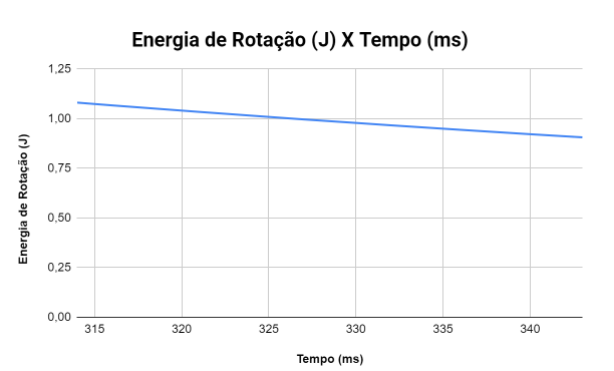
\includegraphics[scale=0.8]{images/energia_de_rotação_x_tempo.png}
  \caption{Energia de Rotação da roda em função do tempo.}
\end{figure}

Com base na Tabela X e no Gráfico 1, podemos determinar a energia média perdida pelo sistema em um ciclo de oscilação:

\[\Delta E = \frac {|E_f - E_i|}{E_i}\cdot 100 = \frac {|0,9060 - 1,0811|}{1,0811} \cdot 100 \]
\[\Delta E = \frac {|-0,1751|}{1,0811}\cdot 100 = 0,1619\cdot 100 \]
\[\Delta E \approx 16\% \]

Portanto, podemos concluir que houve uma variação de cerca de 16\% na Energia de rotação do sistema em um ciclo de oscilação. Isso indubitavelmente poderá interferir nos resultados do experimento, o que já era esperado se levarmos em consideração que há dissipação de energia de atrito durante o experimento. Entretanto, levando em consideração que há um cálculo de variação relativa ao final do experimento e que o experimento é repetido mais de uma vez, podemos utilizar os dados obtidos para uma aproximação de resultados e analisar os conceitos aplicados na prática. Se tratando das equações de conservação de momentum angular, é válido aplicá-las nesse contexto de repetição do experimento e obtenção de mais de um resultado para o cálculo da média.

Feito essa análise, os próximos dados coletados são os relativos às velocidades angulares obtidas imediatamente antes e depois da colisão rotacional. Assumindo que a Peça 2 apresenta velocidade angular inicial igual a zero ($\omega_2$ = 0), que a velocidade imediatamente antes da colisão corresponde à velocidade angular da Peça 1 e que o experimento foi repetido três vezes, temos os dados registrados na Tabela a seguir:

\begin{table}[H]
    \centering
    \begin{tabular}{ |M{5cm}||M{2.5cm}||M{2.5cm}||M{2.5cm}|}
        \hline
        \textbf{} & \textbf{1º Choque Rotacional} & \textbf{2º Choque Rotacional} & \textbf{3º Choque Rotacional}\\
        \hline
        Velocidade Angular Inicial da Peça 1 - $\omega_1$ (rad/s) &  14,444 &  22,765 & 24,353\\
        \hline
        Velocidade Angular Inicial da Peça 2 - $\omega_2$ (rad/s) &  0 &  0 & 0\\
        \hline
        Velocidade Angular Final -$\omega$ (rad/s) &  7,453 &  12,177 & 13,629\\
        \hline
    \end{tabular}
    \caption{Velocidade Angular imediatamente antes e depois da Colisão Rotacional para três repetições.}
\end{table}

Com os dados coletados acima e assumindo que há conservação de Momento Angular durante o experimento com a colisão, calculamos nesse instante o Momento de Inércia  ($I_1$) da Peça 1 através da equação já citada na metodologia:

\[\omega = \frac {I_1\cdot\omega_1 + I_2\cdot\omega_2}{I_1 + I_2}\]
\[I_1 = \frac {\omega - \omega_2}{\omega_1 - \omega}\cdot I_2\]

Como foram realizados três repetições, vamos calcular o momento de inércia da peça 1 para cada um deles:\\

1º) CHOQUE ROTACIONAL
\[I_1 = \frac {7,453 - 0}{14,444 - 7,453}\cdot (0,00522) = 1,066084 \cdot (0,00522) = 0,0055649635 (kg.m^2)\]\\

2º) CHOQUE ROTACIONAL
\[I_1 = \frac {12,177 - 0}{22,765 - 12,177}\cdot (0,00522) = 1,150075 \cdot (0,00522) = 0,0060033944 (kg.m^2)\]\\

3º) CHOQUE ROTACIONAL
\[I_1 = \frac {13,629 - 0}{24,353 - 13,629}\cdot (0,00522) = 1,270888 \cdot (0,00522) = 0,0066340339 (kg.m^2)\]\\

Com os valores calculados para o Momento de Inércia da Peça 1, podemos construir uma tabela que sintetiza os dados obtidos:

\begin{table}[H]
    \centering
    \begin{tabular}{ |M{5cm}||M{2.5cm}||M{2.5cm}||M{2.5cm}|  }
        \hline
        \textbf{ } & \textbf{1º Choque Rotacional} & \textbf{2º Choque Rotacional} & \textbf{3º Choque Rotacional}\\
        \hline
        Momento de Inércia da Peça 1 - $I_1$ (kg.$m^2$)  & 0,0055649635    & 0,0060033944   & 0,0066340339\\
        \hline
    \end{tabular}
    \caption{Momento de Inércia da Peça 1 ($I_1$) para os três Choques Rotacionais.}
\end{table}

Agora, resta determinar a incerteza experimental do Momento de Inércia da peça 1, que pode ser calculada a partir do Desvio Padrão ($\sigma$) dos valores de $I_1$ nas três medidas. Isso acontece, pois, primeiramente, não houve registro das incertezas das velocidades angulares durante o experimento. Sem essa informação, não é possível determinar a propagação de incerteza baseado nas regras convencionais de derivação. O outro motivo pelo qual podemos determinar a incerteza experimental pelo desvio padrão ($\sigma$) está no fato de que não há variação de grandezas envolvidas no cálculo do momento de inércia da peça 1, portanto a manipulação de suas incertezas se dá apenas pela variação dos valores numéricos.

Para determinar o Desvio Padrão (), devemos calcular a média aritmética dos momentos de inércia obtidos nas três repetições e, após isso, aplicar a seguinte fórmula:

\[\sigma = \sqrt{\frac {\sum(I_i - \overline{I})^2}{N-1}}\]

Então,primeiramente, vamos calcular a média aritmética dos três valores obtidos para o Momento de Inércia da peça 1:

\[\overline{I} = \frac{I_1 + I_2 + I_3}{3} = \frac{0,0055649635 + 0,0060033944 + 0,0066340339}{3} = 0,0060674639 (kg.m^2)\]

Com a Média Aritmética I, podemos sintetizar os próximos cálculos para o Desvio Padrão na Tabela a seguir:

\begin{table}[H]
    \centering
    \begin{tabular}{ |M{3cm}||M{3cm}||M{3cm}||M{3cm}|}
        \hline
        \textbf{ } & \textbf{1º Choque Rotacional} & \textbf{2º Choque Rotacional} & \textbf{3º Choque Rotacional}\\
        \hline
        $(I_i - \overline{I})$ & -0,0005025004 & -0,0000640695 & 0,00056657\\
        $(I_i - \overline{I})^2$ & 2,525066 .$10^{-7}$ & 0,041049 .$10^{-7}$ & 3,210015 .$10^{-7}$\\
        $\sum(I_i - \overline{I})^2$ & 5,776082 . $10^{-7}$  & - & -\\
        $\frac {\sum(I_i - \overline{I})^2}{N-1}$ & 2,888. $10^{-7}$ & - & -\\
        $\sqrt{\frac {\sum(I_i - \overline{I})^2}{N-1}}$ & 0,0005374012 & - & -\\
        \hline
    \end{tabular}
    \caption{Dados para a determinação do Desvio Padrão dos valores de $I_1$ nas três medidas.}
\end{table}

Fazendo os devidos arredondamentos para os algarismos significativos, temos que o Desvio Padrão  dos valores de $I_1$ é igual a:

\[\sigma = 0,0005 (kg.m^2)\]

Dessa forma, o Momento de Inércia ( $I_1$) da Peça 1 e sua respectiva incerteza experimental é:

\[\therefore \mathbf{I_1 = (0,0061 \pm 0,0005) kg.m^2}\]\

Por fim, resta calcular as Energias Cinéticas Rotacionais, antes e depois da colisão, e sua variação relativa. Podemos determinar as energias cinéticas a partir das seguintes equações:\\

\[E_{ci} = \frac{1}{2} \cdot I_1 \cdot \omega_1^2\]
\[E_{cf} = \frac{1}{2} \cdot (I_1 + I_2) \cdot \omega_f^2\]

onde $I_1$e $I_2$ são os valores calculados nas etapas anteriores desse experimento, e as velocidades angulares, inicial e final, foram obtidas pelos dados registrados na Tabela. Portanto, teremos o registro de três energias cinéticas iniciais e finais, cada uma com a respectiva velocidade angular:\\

1º) CHOQUE ROTACIONAL\\

A)Energia Cinética Inicial
\[E_{ci} = \frac {1}{2}\cdot (0,0061) \cdot (14,444)^2 = 0,00305 \cdot (208,629136) = 0,6363 J\]

B)Energia Cinética Final
\[E_{cf} = \frac {1}{2}\cdot (0,0061+ 0,005220) \cdot (7,453)^2 = \frac {1}{2}\cdot (0,01132) \cdot 55,547209 = 0,3144 J\]\\

2º) CHOQUE ROTACIONAL\\

C)Energia Cinética Inicial
\[E_{ci} = \frac {1}{2}\cdot (0,0061) \cdot (22,765)^2 = 0,00305 \cdot (518,245225) = 1,5806 J\]

D)Energia Cinética Final
\[E_{cf} = \frac {1}{2}\cdot (0,0061+ 0,005220) \cdot (12,177)^2 = \frac {1}{2}\cdot (0,01132) \cdot 148,279329 = 0,8393 J\]\\

3º) CHOQUE ROTACIONAL\\

E)Energia Cinética Inicial
\[E_{ci} = \frac {1}{2}\cdot (0,0061) \cdot (24,353)^2 = 0,00305 \cdot (593,068609) = 1,8088 J\]

F)Energia Cinética Final
\[E_{cf} = \frac {1}{2}\cdot (0,0061+ 0,005220) \cdot (13,629)^2 = \frac {1}{2}\cdot (0,01132) \cdot 185,749641 = 1,0513 J\]\\

Podemos notar antecipadamente que, ao analisar as energias cinéticas rotacionais iniciais e finais para cada choque, claramente não há conservação de energia. Porém, para uma análise mais completa, calcularemos o Desvio Padrão para as três medidas para, então, comparar se houve ou não conservação de energia. Para isso, retomaremos a fórmula de desvio padrão já utilizado para o Momento de Inércia da peça 1

Então,primeiramente, vamos calcular a média aritmética dos três valores obtidos para a Energia Cinética Rotacional Inicial e para a Energia Cinética Rotacional Final :

\[\overline{E_i} = \frac{0,6363 + 1,5806 + 1,8088}{3} = 1,3419 J\]
\[\overline{E_f} = \frac{0,3144 +  0,8393 + 1,0513}{3} = 0,7350 J\]\\

Com as Médias Aritméticas $\overline{E_i}$ e $\overline{E_f}$, podemos sintetizar os próximos cálculos para o Desvio Padrão nas Tabelas a seguir:

\begin{table}[H]
    \centering
    \begin{tabular}{ |M{3cm}||M{2.8cm}||M{2.8cm}||M{2.8cm}|}
        \hline
        \textbf{ } & \textbf{1º Choque Rotacional} & \textbf{2º Choque Rotacional} & \textbf{3º Choque Rotacional}\\
        \hline
        $(E_i - \overline{E})$                                        & -0,7056    & 0,2387  & 0,4669\\
        $(E_i - \overline{E})^2$                                      & 0,49787136    & 0,05697769  & 0,21799561\\
        $\sum(E_i - \overline{E})^2$                                  & 0,77284466  &    & \\
        $\frac {\sum(E_i - \overline{E})^2}{N-1}$                     & 0,38642233   &    &\\
        $\sqrt{\frac {\sum(E_i - \overline{E})^2}{N-1}}$              & 0,6216287719   &    &\\
        \hline
    \end{tabular}
    \caption{Dados para a determinação do Desvio Padrão dos valores da Energia Cinética Rotacional Inicial $E_i$ nas três medidas.}
\end{table}

\begin{table}[H]
    \centering
    \begin{tabular}{ |M{3cm}||M{2.8cm}||M{2.8cm}||M{2.8cm}|}
        \hline
        \textbf{ } & \textbf{1º Choque Rotacional} & \textbf{2º Choque Rotacional} & \textbf{3º Choque Rotacional}\\
        \hline
        $(E_f - \overline{E})$                                        & -0,4206    & 0,1043  & 0,3163\\
        $(E_f - \overline{E})^2$                                      & 0,17690436    & 0,0108749  & 0,10004569\\
        $\sum(E_f - \overline{E})^2$                                  & 0,28782854  &    & \\
        $\frac {\sum(E_f - \overline{E})^2}{N-1}$                     & 0,14391427   &    &\\
        $\sqrt{\frac {\sum(E_f - \overline{E})^2}{N-1}}$              & 0,3793603432   &    &\\
        \hline
    \end{tabular}
    \caption{Dados para a determinação do Desvio Padrão dos valores da Energia Cinética Rotacional Final $E_f$ nas três medidas.}
\end{table}

Fazendo os devidos arredondamentos para os algarismos significativos, temos que o Desvio Padrão  dos valores de $E_{inicial}$ e $E_{final}$ são iguais a:

\[\sigma_{inicial} = 0,6 J\]
\[\sigma_{final} = 0,4 J\]

Dessa forma, as Energia Cinética Rotacional Inicial ( $E_i$) e a Energia Cinética Rotacional Final ( $E_f$), com suas respectivas incertezas experimental, são:

\[\mathbf{E_i = (1,3 \pm 0,6) J}\]\
\[\mathbf{E_f = (0,7 \pm 0,4) J}\]\

Com esses valores calculados, podemos determinar a Variação Relativa para então analisar se houve ou não conservação de energia durante o experimento. A Variação Relativa pode ser calculado fazendo a divisão da variação de energia pela energia inicial:

\[\Delta E_c (\%) = 100 \cdot \frac{|E_{ci} - E_f|}{E_{ci}}\]
\[\Delta E_c (\%) = 100 \cdot \frac{|1,3 - 0,7|}{1,3} = 100 \cdot 0,461538\]
\[\mathbf{\Delta E_c (\%) = 46(\%)}\]\

Então, podemos concluir que houve uma variação de aproximadamente 46\% se compararmos as Energias Cinéticas Rotacionais inicial e final. Isso representa uma não conservação de energia, pois da quantidade de energia presente no início do experimento, cerca de 46\% se dissiparam em alguma outra forma de energia. Isso pode ser justificado por alguns motivos: o primeiro deles está no fato do experimento envolver atrito entre o eixo de rotação e as peças girando, o que ocasiona uma dissipação de parte da energia; além disso, o choque em questão representa um choque perfeitamente inelástico (os corpos seguem juntos após a colisão com a mesma velocidade) que, por característica, não conserva a energia mecânica.

Podemos sintetizar todos os dados relevantes desse experimento na seguinte Tabela X a seguir: 

\begin{table}[H]
    \centering
    \begin{tabular}{ |M{1.6cm}||M{1.5cm}||M{1.5cm}||M{1.6cm}||M{1.9cm}||M{1.3cm}||M{1.3cm}||M{1cm}|}
        \hline
        \textbf{Nº Choque} & \textbf{$\omega_1$ (rad/s)} & \textbf{$\omega_f$ (rad/s)} & \textbf{$I_1$ (kg.$m^2$)} & \textbf{$I_2$ (kg.$m^2$)} & \textbf{$E_{ci}$ (J)} & \textbf{$E_{cf}$ (J)} & \textbf{$\Delta E_c$ (\%)}\\
        \hline
        1 & 14,444 & 7,453 & - & - & - & - & -\\
        2 & 22,765 & 12,177 & 0,0061 $\pm$ 0,0005 & 0,00522 $\pm$ 0,00002 & 1,3 $\pm$ 0,6 & 0,7 $\pm$ 0,4 & 46\%\\
        3 & 24,353 & 13,629 & - & - & - & - & -\\
        \hline
    \end{tabular}
    \caption{Valores obtidos no experimento de Choque Rotacional.}
\end{table}

Comparando o valor obtido para o momento de Inércia da peça 1 ($I_1 = 0,0061 \pm 0,0005$) com os valores obtidos a partir das características geométricas e do experimento com a roda de Maxwell ($I_1 = 0,00540 \pm 0,00005$ e $I_F = 0,00497 \pm 0,00002$), podemos observar que 
